\documentclass[a4paper,10pt]{article}
\usepackage[utf8]{inputenc}
\usepackage{subcaption}
\usepackage{listings}
\usepackage{color}
\usepackage{gensymb}
\usepackage{graphicx}
\usepackage{minted}
\usepackage{float}
\definecolor{codegreen}{rgb}{0,0.6,0}
\definecolor{codegray}{rgb}{0.5,0.5,0.5}
\definecolor{codepurple}{rgb}{0.58,0,0.82}
\definecolor{backcolour}{rgb}{0.95,0.95,0.92}
\usepackage{geometry}
\geometry{hmargin=2.5cm}
\usepackage{hyperref}
\usepackage{xcolor}
\usepackage{tcolorbox}

\lstdefinestyle{mystyle}{
    backgroundcolor=\color{backcolour},   
    commentstyle=\color{codegreen},
    keywordstyle=\color{magenta},
    numberstyle=\tiny\color{codegray},
    stringstyle=\color{codepurple},
    basicstyle=\footnotesize,
    breakatwhitespace=false,         
    breaklines=true,                 
    captionpos=b,                    
    keepspaces=true,                 
    numbers=left,                    
    numbersep=5pt,                  
    showspaces=false,                
    showstringspaces=false,
    showtabs=false,                  
    tabsize=2
}
\lstset{style=mystyle}

\definecolor{OliveGreen}{rgb}{.1,.6,.1}
\definecolor{backgroundItem}{RGB}{41,44,52}
\definecolor{TypeItem}{RGB}{203, 154, 204}
\definecolor{NameItem}{RGB}{247, 196, 94}
\definecolor{DescriptionItem}{RGB}{128, 197, 154}
\definecolor{GroupItem}{RGB}{238, 140, 80}
\definecolor{FuncItem}{RGB}{224, 119, 123}

\tcbset{width=0.9\textwidth,boxrule=0pt,colback=backgroundItem,arc=10pt,auto outer arc,left=0pt,right=0pt,boxsep=5pt}

\title{Eclipse Smarthome \\ IOTA Integration}
\author{Théo Giovanna}
\date{May 2018}

\begin{document}

\maketitle

\section{Global Configuration}

\subsection{Metadata}

This add-on allows you to expose your SmartHome system to the IOTA blockchain, \textbf{Tangle}.
Using this add-on, you will be able to configure for each \textit{Thing} of your choice some \textit{metadata}. Metadata are extra-information that can be attached to an \textit{item}. This add-on offers two types of metadata: \\

\begin{itemize}
	\item \texttt{value:} \textit{"yes"} | \texttt{label:} \textit{"Share the item's state with the Tangle"}
	\item \texttt{value:} \textit{"no"} | \texttt{label:} \textit{"Don't share the item's state with the Tangle"}
\end{itemize} 

\noindent The \textit{"yes"} value allows for some more fine tuning:

\begin{itemize}
	\item \texttt{param:} \textit{"mode"} | \texttt{public, private, restricted}
	\item \texttt{param:} \textit{"key"} | \texttt{Optional key for restricted mode}
	\item \texttt{param:} \textit{"seed"} | \texttt{Optional seed. Allows one to publish on an existing channel}
\end{itemize}

\bigskip

\noindent For information about what \textit{Things}, \textit{Channels} and \textit{Items} are, please refer to the official \textcolor{blue}{\underline{\href{https://www.eclipse.org/smarthome/documentation/index.html}{ESH documentation}}}. To be able to configure metadata for your items, you must ensure that the option \texttt{Simple Mode} under \texttt{Configuration > System > Item Linking} is turned off.

\subsection{IOTA}

\noindent Besides configuring the Item metadata, one must configure the IOTA API settings, by which information will transit. As described in the \textcolor{blue}{\underline{\href{https://github.com/iotaledger/iota.lib.java}{JAVA wrapper documentation for IOTA}}}, an \texttt{\textcolor{red}{IotaAPI}} instance must be created in order to interact with the Tangle. This instance has three settings: \textit{protocol, host, port}. By default, this add-on is configured with the following settings: \\

\begin{itemize}
	\item Protocol: \texttt{https}
	\item Host: \texttt{nodes.tangle.testnet.iota.org}
	\item Port: \texttt{443}
\end{itemize} 

\bigskip

\noindent Each one of these settings can be edited at any time through the PaperUI, under \texttt{Configuration > Services}. You are free to use any remote nodes running the IOTA protocol, as well as local nodes. 

\section{Technical information}

The purpose of this section is to describe how the add-on works, as well as giving some hints on why IOTA was chosen and how this can be beneficial for your smart home system.

\subsection{The Tangle}

The Tangle isn’t a blockchain per se, as it is block-less. Instead of miners solving cryptographic puzzles in order to verify new blocks, the Tangle is quite different: there are no miners. Instead, the users themselves verify the transaction: to create a new transaction, one needs to validate two other transactions. This has the additional benefit of speeding up the network the more one uses it. Moreover, Tangle is fee-less which makes it a perfect fit for micro-transactions. IOTA is the name of the cryptocurrency that is based upon Tangle. \\

\noindent In a world where the \textit{Internet of Things}, or \textit{IoT}, is taking more and more breadth, the Tangle has a key role to play. The main challenge isn’t in creating smart devices or machines, but rather it is at the communication level. The Tangle enables a future in which devices can securely communicate with and autonomously compensate each other. For more information on how the Tangle works at his core, I encourage you to read this \textcolor{blue}{\underline{\href{https://blog.iota.org/the-tangle-an-illustrated-introduction-4d5eae6fe8d4}{series of articles}}} published on their blog. You can also view their official white-paper \textcolor{blue}{\underline{\href{http://iotatoken.com/IOTA_Whitepaper.pdf}{here}}}. 

\subsection{ESH IOTA Add-on}

The basic idea behind this add-on is to use the Tangle capabilities in order to share any item's state on it. Lately, IOTA revealed a new feature running on the Tangle: \textbf{Masked Authenticated Messaging}, or MAM for short. MAM is a second layer data communication protocol which adds functionality to emit and access an encrypted data stream, like RSS, over the Tangle, regardless of the size or cost of device. IOTA’s consensus protocol adds integrity to these message streams. Information on MAM can be found on their official \textcolor{blue}{\underline{\href{https://blog.iota.org/introducing-masked-authenticated-messaging-e55c1822d50e}{blog}}}. This add-on therefore uses MAM as a mean of communication between any ESH thing (providers) and entities that want to know the states of these things (subscribers). 

\subsubsection{Publishing an item's state to the Tangle}

The iota add-on implements several interfaces from ESH, some of which are enumerated and explained below:

\begin{itemize}
	\item \texttt{\textcolor{red}{RegistryChangeListener<Metadata>}}, implemented by \texttt{\textcolor{OliveGreen}{IotaMetadataRegistryChangeListener}}: Each time a metadata is added, updated or removed, the implementing class is notified.
	\item \texttt{\textcolor{red}{ItemRegistryChangeListener}}, implemented by \texttt{\textcolor{OliveGreen}{IotaItemRegistryListener}}: Each time an item is added, updated or removed, the implementing class is notified.
	\item \texttt{\textcolor{red}{StateChangeListener}}, implemented by \texttt{\textcolor{OliveGreen}{IotaItemStateChangeListener}}: Each time an item sees its state changed or updated, the implementing class if notified. 
	\item \texttt{\textcolor{red}{MetadataConfigDescriptionProvider}}, implemented by \texttt{\textcolor{OliveGreen}{IotaMetadataProvider}}: Allows one to offer different configuration for metadata in the PaperUI.
\end{itemize}

\noindent The flow is therefore as follow: anytime one adds metadata to an existing item offered by this add-on or that a new item is created with metadata "iota" with value "yes", the add-on will pick up the event and monitor future state changes of this item, by associating to it a \texttt{StateListener} as described above. \\

\noindent For instance, consider the following item, defined in \texttt{demo.items}:

\begin{center}
\begin{tcolorbox}
\textcolor{TypeItem}{Number}\textcolor{white}{:}\textcolor{TypeItem}{Temperature} \textcolor{NameItem}{Weather\_Temperature} \textcolor{DescriptionItem}{"OutsideTemperature[\%.1f\degree C]"}\textcolor{GroupItem}{$<$temperature$>$} \textcolor{FuncItem}{(Weather\_Chart)} \textcolor{white}{\{iota=}\textcolor{DescriptionItem}{"yes"} \textcolor{white}{[mode=}\textcolor{DescriptionItem}{"public"}\textcolor{white}{,} \textcolor{white}{seed=}\textcolor{DescriptionItem}{"yourSeed"}\textcolor{white}{,} \textcolor{white}{key=}\textcolor{DescriptionItem}{"null"}\textcolor{white}{]}\textcolor{white}{,} \\ \textcolor{white}{channel=} \textcolor{DescriptionItem}{"yahooweather:weather:berlin:temperature"} \textcolor{white}{\}}
\end{tcolorbox}

\end{center}

\noindent And in \texttt{demo.things}:

\begin{center}
\begin{tcolorbox}
\textcolor{TypeItem}{yahooweather}\textcolor{white}{:}\textcolor{TypeItem}{weather}\textcolor{white}{:}\textcolor{NameItem}{berlin} \textcolor{GroupItem}{[ location=638242 ]}
\end{tcolorbox}
\end{center}

\noindent MAM allows for three different publishing modes: \texttt{public, private, restricted}. These options can be configured in PaperUI through metadata. More information on what achieves each mode can be found in the blog link given above. Each item may also be published on a given MAM channel, through \textit{seeds}. In such scenario, the flow is as follow: let $X$ be an ESH instance with items $A, B, C, D$. Let $Y$ and $Z$ be to other ESH instances. $X$ may choose to share on a \texttt{public, private or restricted} channel $A$ and $B$'s state with $Y$. Therefore, all states will be published on seed $s_0$ with root $r_0$. Now, $X$ may also choose to share with $Z$ on a separate channel (\texttt{public, private or restricted}) $C$ and $D$'s state, on seed $s_1$. $X$ is now broadcasting data on two different channels, each belonging to a seed: $s_0, s_1$. To add new item's state to any of these streams, say the first one broadcasting to $Y$, $X$ just has to configure a new item's metadata with the seed he's using for $Y$, in this case $s_0$. \\ 

\noindent In the previously defined item, we defined the metadata \texttt{"iota=yes"} with several parameters. The add-on will detect it and associate a state listener to this item. From now on, every update of this item will be detected and pushed on the Tangle. In MAM, the first transaction emitted has a \texttt{Root} address, which is derived from the \textbf{seed}. Any sub-sequent message (i.e. any new update on the item's state) will be published on the \texttt{NextRoot} address, which is contained in any transaction retrieved from MAM. Given the first \texttt{root} address, or any \texttt{nextRoot} address that follows, one can see all the states shared from this address onward using the \textcolor{blue}{\underline{\href{https://mam-explorer.firebaseapp.com/}{official MAM-Explorer}}}. For instance:

\begin{figure}[H]
  \center
  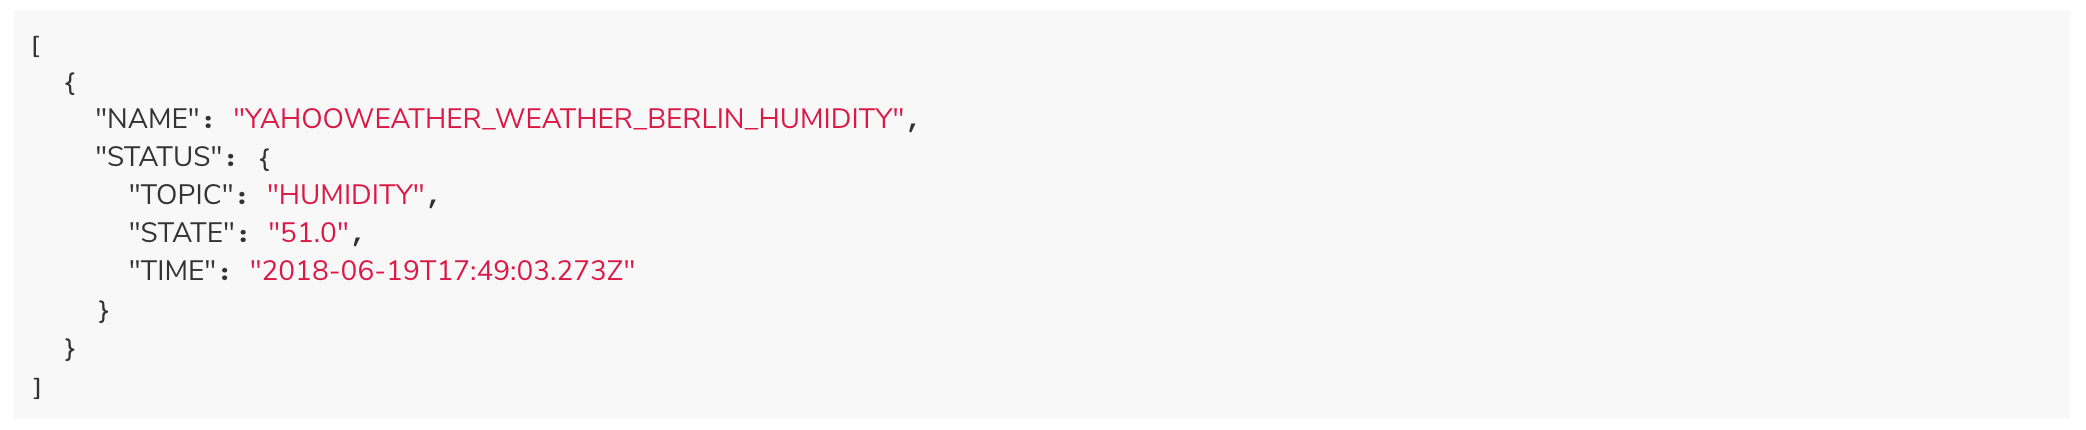
\includegraphics[scale=0.50]{images/mam_retrieve.png}
  \captionof{figure}{Retrieving item states through MAM}
\end{figure}

\newpage 

\section{Javadoc}

\textbf{Note:} getters and setters are left out of this java documentation, which is here just to give the user a grasp of how this add-on is organized and what are the responsibilities of each class.

\subsection{\texttt{Debouncer.java}}

\begin{minted}[frame=single,framesep=10pt]{java}
/**
 * Implements a debounce mechanism.
 *
 * @author Theo Giovanna - Initial Contribution
 */
public class Debouncer {
	/**
	 * Debounces {@code callable} by {@code delay}, i.e., schedules it to be
	 * executed after {@code delay}, or cancels its execution if the method 
	 * is called with the same key within the {@code delay} again. 
	 * @author simon04 
	 * https://stackoverflow.com/questions/4742210/implementing-debounce-in-java
	 */
	 public void debounce(final Object key, final Runnable runnable, long delay,
	 TimeUnit unit) {}
}
\end{minted}

\subsection{\texttt{Iota.java}}

\begin{minted}[frame=single,framesep=10pt]{java}
/**
 * Set up the IOTA API and the metadata listener
 * @author Theo Giovanna - Initial Contribution
 */
public class Iota {
	
    protected synchronized void activate(Map<String, Object> data) {}
    protected void deactivate() {}
    
    /**
     * This function is called every time that the user updates the API parameters
     * in Paper UI. The Iota API instance is then updated accordingly
     */
    protected synchronized void modified(IotaApiConfiguration config) {}
    
    /**
     * Called when the component is started. Set up the IOTA API
     */
    private void start() {}
}
\end{minted}


\subsection{\texttt{IotaApiConfiguration.java}}

\begin{minted}[frame=single,framesep=10pt]{java}
/**
 * Configuration parameters of the {@link Iota}.
 * @author Theo Giovanna - Initial Contribution
 */
public class IotaApiConfiguration {

}
\end{minted}

\subsection{\texttt{IotaItemRegistryChangeListener.java}}

\begin{minted}[frame=single,framesep=10pt]{java}
/**
 * Listens for changes to the item registry.
 * @author Theo Giovanna - Initial Contribution
 */
public class IotaItemRegistryChangeListener implements ItemRegistryChangeListener {

	/**
	 * Called when items are added, removed or updated
	 */ 
	public void added(Item element) {}
	public void removed(Item element) {}
	public void updated(Item oldElement, Item element) {}
	public void allItemsChanged(Collection<String> oldItemNames) {}

	/**
	 * Add a registry change listener
	 */
	public synchronized void setItemRegistry(ItemRegistry itemRegistry) {}

}
\end{minted}

\newpage

\subsection{\texttt{IotaItemStateChangeListener.java}}

\begin{minted}[frame=single,framesep=10pt]{java}
/**
 * Listens for changes to the state of registered items.
 * Each item wishing to publish its state on the Tangle has a seed associated to its 
 * UID. A custom seed may be given to some item. This way, any ESH instance is able 
 * to select which item's state to share on which channel.
 * @author Theo Giovanna - Initial Contribution
 */
public class IotaItemStateChangeListener implements StateChangeListener {

	/**
	 * Called when a registered item sees its state changed or updated
	 */ 
	public void stateChanged(@NonNull Item item, @NonNull State oldState, 
	@NonNull State newState) {}
	public void stateUpdated(@NonNull Item item, @NonNull State state) {}
	
	/**
	 * Constructs a JSON object with all item names and states that will
	 * be published on the Tangle.
	 */
	 public synchronized void addToStates(@NonNull Item item, 
	 @NonNull State state) {}
	 
	 /**
	 * Cleaning json struct: an item has been removed in the Paper UI, therefore 
	 * its state will not be published to the Tangle anymore
	 */
	 public void removeItemFromJson(@NonNull Item item) {}

}
\end{minted}

\subsection{\texttt{IotaMetadataProvider.java}}

\begin{minted}[frame=single,framesep=10pt]{java}
/**
 * Describes the metadata for the "iota" namespace.
 * @author Theo Giovanna - initial contribution
 */
public class IotaMetadataProvider implements MetadataConfigDescriptionProvider {

}

\end{minted}

\newpage

\subsection{\texttt{IotaMetadataRegistryChangeListener.java}}

\begin{minted}[frame=single,framesep=10pt]{java}
/**
 * Listens for changes to the metadata registry.
 * This class will allow items to be listened to through the
 * IotaItemStateChangeListener class if they contain the metadata IOTA, when
 * created.
 * @author Theo Giovanna - Initial Contribution
 */
public class IotaMetadataRegistryChangeListener implements RegistryChangeListener<Metadata> {
	
	/**
	 * Called when metadata are added, removed or updated
	 */ 
	public void added(Metadata element) {}
	public void removed(Metadata element) {}
	public void updated(Metadata oldElement, Metadata element) {}
	
	/**
	* Updates the hashmaps in the {@link IotaStateListener} class.
	*/
	public void updateMaps(Item item, String seed) {}
    
	/**
	 * Add a registry change listener
	 */
	public void setMetadataRegistry(MetadataRegistry metadataRegistry) {}
	
	/**
	 * Remove the registry change listener
	 */
	public void stop() {}
	
}

\end{minted}

\newpage 

\subsection{\texttt{IotaSettings.java}}

\begin{minted}[frame=single,framesep=10pt]{java}
/**
 * Provides the configured and static settings for the IOTA add-on
 * @author Theo Giovanna - Initial Contribution
 */
public class IotaSettings {

	/**
	 * Sets the config. parameters
	 * Adapted from org.openhab.io.homekit.internal
	 * @author Andy Lintner
	 */
	public void fill(IotaApiConfiguration config) throws UnknownHostException {}
	private static String getOrDefault(Object value, String defaultValue) {}
}

\end{minted}

\subsection{\texttt{IotaUtils.java}}

\begin{minted}[frame=single,framesep=10pt]{java}
/**
 * Provides utils methods to work with IOTA transactions
 * @author Theo Giovanna - Initial Contribution
 */
public class IotaUtils {
	/**
	 * Attach an item's state to the Tangle
	 */
	protected void publishState(JsonElement jsonElement, String mode, 
	String key) {}
	/**
	 * Retrieve an item state from the Tangle, through MAM
	 */
	 public String fetchFromTangle(int refresh, String root, String mode) {} 
	/**
	 * Checks the IOTA API
	 */
	 public boolean checkAPI() {}
	 /**
	 * Check the validity of a seed
	 */
	 public boolean checkSeed(String seed) {}
}
\end{minted}

\end{document}